\documentclass{beamer}
\usepackage[utf8]{inputenc}
\usepackage[french]{babel}
\usepackage{setspace}
\usepackage{hyperref}
\usepackage{amsmath}
\usepackage{pifont}
\usepackage{color}
\usetheme{AnnArbor}
% Just add % Just add % Just add \input{smalltalkEnv} to your file
% then you can use :
% \begin{lstlisting}[language=Smalltalk]
% false become: true.
% \end{lstlisting}

\usepackage{color}
\usepackage{listings}
\usepackage{etoolbox}
\usepackage{textcomp}

\definecolor{stComment}{rgb}{0.5,0.5,0.5}
\definecolor{stString}{rgb}{0.58,0,0.82}
\definecolor{stKeywords}{rgb}{0.21,0.55,0.7}
\definecolor{stNumbers}{rgb}{.5,0,0}

\newtoggle{InString}{}% Keep track of if we are within a string
\togglefalse{InString}% Assume not initally in string
\newcommand*{\ColorIfNotInString}[1]{\iftoggle{InString}{#1}{\color{stNumbers}#1}}%
\newcommand*{\ProcessQuote}[1]{#1\iftoggle{InString}{\global\togglefalse{InString}}{\global\toggletrue{InString}}}%

\lstdefinelanguage{Smalltalk}{
  keywordstyle=\color{stKeywords},
  commentstyle=\color{stComment},
  stringstyle=\color{stString},
  alsoletter=\#,
  identifierstyle=\idstyle, 
  showstringspaces=false,
  morekeywords={true,false,self,super,nil},
  sensitive=true, 
  morecomment=[s]{"}{"}, 
  morestring=[d]', 
  style=SmalltalkStyle,
  tabsize=2,
  basicstyle=\ttfamily,
  upquote=true,
}


\makeatletter%
\newcommand*\idstyle[1]{%
  \expandafter\id@style\the\lst@token{#1}\relax%
}
\def\id@style#1#2\relax{%
  \ifnum\pdfstrcmp{#1}{\#}=0%
  \ttfamily\color{stString} \the\lst@token%
  \else%
  \edef\tempa{\uccode`#1}%
  \edef\tempb{`#1}%
  \ifnum\tempa=\tempb%
  \ttfamily\color{blue} \the\lst@token%
  \else%
  \the\lst@token%
  \fi%
  \fi%
}

\lstdefinestyle{SmalltalkStyle}{ 
  literate=%
  {^}{{$\uparrow$}}1% 
  % {"}{{{\ProcessQuote{"}}}}1% Disable coloring within double quotes
  % {'}{{{\ProcessQuote{'}}}}1% Disable coloring within single quote
  {0}{{{\ColorIfNotInString{0}}}}1%
  {1}{{{\ColorIfNotInString{1}}}}1%
  {2}{{{\ColorIfNotInString{2}}}}1%
  {3}{{{\ColorIfNotInString{3}}}}1%
  {4}{{{\ColorIfNotInString{4}}}}1%
  {5}{{{\ColorIfNotInString{5}}}}1%
  {6}{{{\ColorIfNotInString{6}}}}1%
  {7}{{{\ColorIfNotInString{7}}}}1%
  {8}{{{\ColorIfNotInString{8}}}}1%
  {9}{{{\ColorIfNotInString{9}}}}1%
} 
 to your file
% then you can use :
% \begin{lstlisting}[language=Smalltalk]
% false become: true.
% \end{lstlisting}

\usepackage{color}
\usepackage{listings}
\usepackage{etoolbox}
\usepackage{textcomp}

\definecolor{stComment}{rgb}{0.5,0.5,0.5}
\definecolor{stString}{rgb}{0.58,0,0.82}
\definecolor{stKeywords}{rgb}{0.21,0.55,0.7}
\definecolor{stNumbers}{rgb}{.5,0,0}

\newtoggle{InString}{}% Keep track of if we are within a string
\togglefalse{InString}% Assume not initally in string
\newcommand*{\ColorIfNotInString}[1]{\iftoggle{InString}{#1}{\color{stNumbers}#1}}%
\newcommand*{\ProcessQuote}[1]{#1\iftoggle{InString}{\global\togglefalse{InString}}{\global\toggletrue{InString}}}%

\lstdefinelanguage{Smalltalk}{
  keywordstyle=\color{stKeywords},
  commentstyle=\color{stComment},
  stringstyle=\color{stString},
  alsoletter=\#,
  identifierstyle=\idstyle, 
  showstringspaces=false,
  morekeywords={true,false,self,super,nil},
  sensitive=true, 
  morecomment=[s]{"}{"}, 
  morestring=[d]', 
  style=SmalltalkStyle,
  tabsize=2,
  basicstyle=\ttfamily,
  upquote=true,
}


\makeatletter%
\newcommand*\idstyle[1]{%
  \expandafter\id@style\the\lst@token{#1}\relax%
}
\def\id@style#1#2\relax{%
  \ifnum\pdfstrcmp{#1}{\#}=0%
  \ttfamily\color{stString} \the\lst@token%
  \else%
  \edef\tempa{\uccode`#1}%
  \edef\tempb{`#1}%
  \ifnum\tempa=\tempb%
  \ttfamily\color{blue} \the\lst@token%
  \else%
  \the\lst@token%
  \fi%
  \fi%
}

\lstdefinestyle{SmalltalkStyle}{ 
  literate=%
  {^}{{$\uparrow$}}1% 
  % {"}{{{\ProcessQuote{"}}}}1% Disable coloring within double quotes
  % {'}{{{\ProcessQuote{'}}}}1% Disable coloring within single quote
  {0}{{{\ColorIfNotInString{0}}}}1%
  {1}{{{\ColorIfNotInString{1}}}}1%
  {2}{{{\ColorIfNotInString{2}}}}1%
  {3}{{{\ColorIfNotInString{3}}}}1%
  {4}{{{\ColorIfNotInString{4}}}}1%
  {5}{{{\ColorIfNotInString{5}}}}1%
  {6}{{{\ColorIfNotInString{6}}}}1%
  {7}{{{\ColorIfNotInString{7}}}}1%
  {8}{{{\ColorIfNotInString{8}}}}1%
  {9}{{{\ColorIfNotInString{9}}}}1%
} 
 to your file
% then you can use :
% \begin{lstlisting}[language=Smalltalk]
% false become: true.
% \end{lstlisting}

\usepackage{color}
\usepackage{listings}
\usepackage{etoolbox}
\usepackage{textcomp}

\definecolor{stComment}{rgb}{0.5,0.5,0.5}
\definecolor{stString}{rgb}{0.58,0,0.82}
\definecolor{stKeywords}{rgb}{0.21,0.55,0.7}
\definecolor{stNumbers}{rgb}{.5,0,0}

\newtoggle{InString}{}% Keep track of if we are within a string
\togglefalse{InString}% Assume not initally in string
\newcommand*{\ColorIfNotInString}[1]{\iftoggle{InString}{#1}{\color{stNumbers}#1}}%
\newcommand*{\ProcessQuote}[1]{#1\iftoggle{InString}{\global\togglefalse{InString}}{\global\toggletrue{InString}}}%

\lstdefinelanguage{Smalltalk}{
  keywordstyle=\color{stKeywords},
  commentstyle=\color{stComment},
  stringstyle=\color{stString},
  alsoletter=\#,
  identifierstyle=\idstyle, 
  showstringspaces=false,
  morekeywords={true,false,self,super,nil},
  sensitive=true, 
  morecomment=[s]{"}{"}, 
  morestring=[d]', 
  style=SmalltalkStyle,
  tabsize=2,
  basicstyle=\ttfamily,
  upquote=true,
}


\makeatletter%
\newcommand*\idstyle[1]{%
  \expandafter\id@style\the\lst@token{#1}\relax%
}
\def\id@style#1#2\relax{%
  \ifnum\pdfstrcmp{#1}{\#}=0%
  \ttfamily\color{stString} \the\lst@token%
  \else%
  \edef\tempa{\uccode`#1}%
  \edef\tempb{`#1}%
  \ifnum\tempa=\tempb%
  \ttfamily\color{blue} \the\lst@token%
  \else%
  \the\lst@token%
  \fi%
  \fi%
}

\lstdefinestyle{SmalltalkStyle}{ 
  literate=%
  {^}{{$\uparrow$}}1% 
  % {"}{{{\ProcessQuote{"}}}}1% Disable coloring within double quotes
  % {'}{{{\ProcessQuote{'}}}}1% Disable coloring within single quote
  {0}{{{\ColorIfNotInString{0}}}}1%
  {1}{{{\ColorIfNotInString{1}}}}1%
  {2}{{{\ColorIfNotInString{2}}}}1%
  {3}{{{\ColorIfNotInString{3}}}}1%
  {4}{{{\ColorIfNotInString{4}}}}1%
  {5}{{{\ColorIfNotInString{5}}}}1%
  {6}{{{\ColorIfNotInString{6}}}}1%
  {7}{{{\ColorIfNotInString{7}}}}1%
  {8}{{{\ColorIfNotInString{8}}}}1%
  {9}{{{\ColorIfNotInString{9}}}}1%
} 



% My preferences
\graphicspath{{images/}}
\newcommand{\tip}{\boldmath{\textcolor{red}{$\Rightarrow$}}}
\newcommand{\drgeo}{Dr.~Geo}
\newcommand{\cmark}{\text{\ding{51}}}
\newcommand{\xmark}{\text{\ding{55}}}

\title{Kids Programming\\ with\\ Smalltalk}
\author{Hilaire Fernandes}
\institute[DIP, Geneva]{Department of Public Instruction \\ Geneva}
\titlegraphic{
  
\includegraphics[width=2cm]{ArmoirieGeneve.png}
}
\date{November 2023}
\begin{document}

\begin{frame}
  \titlepage
\end{frame}
%
\begin{frame}{About me}
  \fontsize{12pt}{30pt}\selectfont
  \begin{itemize}
  \item Educator in public school, Geneva, B.Math, Ma.Ed
  \item Computer scientist, Ma.CS, PhD.CS
  \item Free software enthusiast and user since 1998
  \item And of course, Smalltalk user since 2002
  \end{itemize}
\end{frame}
%
\begin{frame}{Contents}
  \tableofcontents[hideallsubsections]
\end{frame}


\section{Why this presentation?}
\subsection{1. Recent (r)evolution of Cuis}
\begin{frame}[fragile]{Morphic 3}
Mature, Simplified, Understandable and Vector quality!
\begin{columns}[c]
  \begin{column}{0.5\textwidth}
    \fontsize{9pt}{8pt}\selectfont
    \begin{lstlisting}[language=Smalltalk]
DyViewerVisitor>>visitCourse: course
	| column |
	visitedModel := course.
	column := LayoutMorph newColumn.
	column
        addMorph: (self
           paneFor: course courseHours
           label: 'Periods' translated
           browse: false);
        addMorph: (self
           paneFor: course teacher
           label: 'Teacher' translated
           browse: false);
        addMorph: (self
           paneFor: course topics
           label: 'Topics' translated
           browse: false).
	^ self plugView: column
      \end{lstlisting}
    \end{column}    
    \begin{column}{0.5\textwidth}
      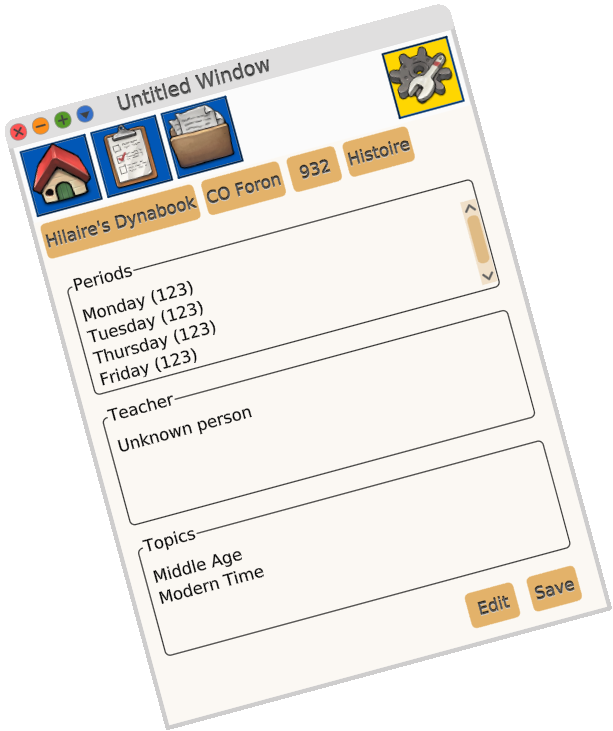
\includegraphics[width=0.9\textwidth]{CompiledLayout.png}
    \end{column}  
  \end{columns}
\end{frame}
%
\begin{frame}[fragile]{Vector Graphics}
 Mature too, API \textsc{svg} compatible. Fast!
  \vspace{0.5cm}
  \begin{columns}[c]
  \begin{column}{0.5\textwidth}
\fontsize{8pt}{0pt}\selectfont
\begin{lstlisting}[language=Smalltalk]
ProtractorMorph>>drawOn: canvas
|  p1 p2 |
canvas
   strokeWidth: 1
   color: Color black
   do: [
     canvas moveTo: 0 @ -0.5;
     lineTo: 0 @ -8].
     
-180 to: 0 do: [:degree |
  canvas strokeWidth: 0.5 color: Color black do: [:engine |
  p1 := Point
    r: 100
    degrees: degree.
  p2 := Point
     r: 95
     degrees: degree.
  engine moveTo: p1 ; lineTo: p2]]
\end{lstlisting}
\end{column} 
  \begin{column}{0.5\textwidth}
    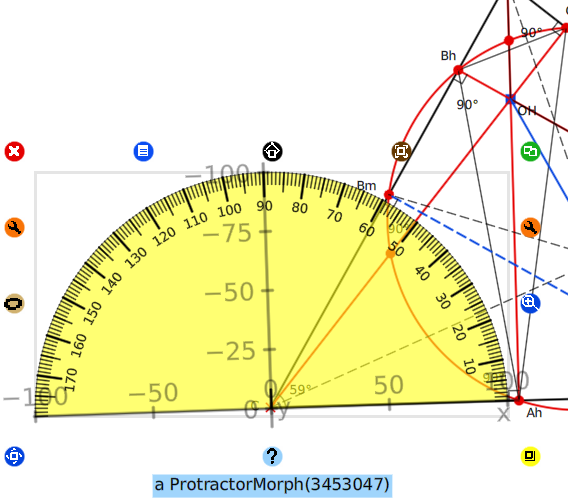
\includegraphics[width=0.9\textwidth]{VectorGraphics.png}
  \end{column}  
\end{columns}
\end{frame}
%
\begin{frame}{Unicode}
  \begin{columns}[c]
    \begin{column}{0.5\textwidth}
      \begin{itemize}
      \item The default encoding for source code, text and text files
      \item Methods can be nammed with Unicode symbols
      \item Variables too !
      \end{itemize}
    \end{column}
    \begin{column}{0.5\textwidth}
      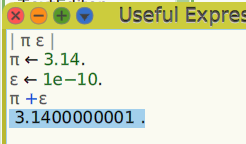
\includegraphics[width=0.7\textwidth]{unicodeInCode.png}      
    \end{column}
  \end{columns}
\end{frame}
%
\begin{frame}[fragile]{Packaging System}
  \begin{columns}[c]
    \begin{column}{0.5\textwidth}
      \fontsize{8pt}{0pt}\selectfont
      \begin{lstlisting}[language=Smalltalk]
        "Install DrGeo code"
        Feature require: #'DrGeo'.
        Feature require: #'DrGeoFrench'.
      \end{lstlisting}      
    \end{column}
    \begin{column}{0.5\textwidth}
      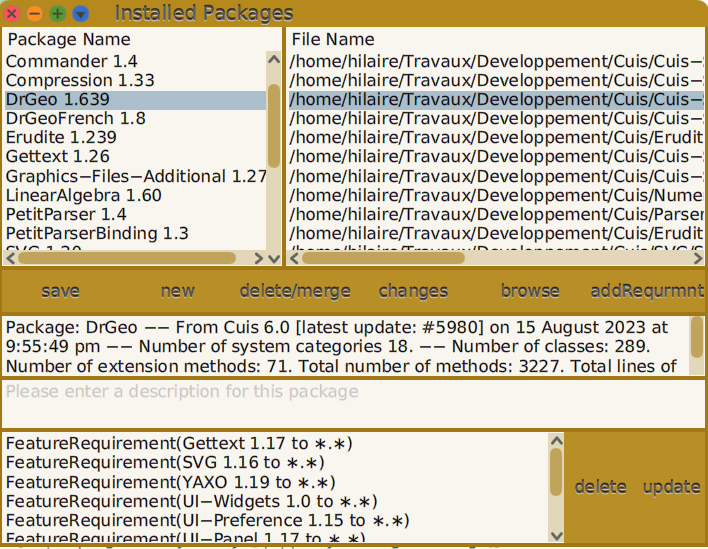
\includegraphics[width=\textwidth]{codePackager.png}       
    \end{column}
  \end{columns}
\end{frame}

\subsection{2. GUI application with Smalltalk}
\begin{frame}
Example of fine tuned end-user application with \alert{Smalltalk}!
\begin{itemize}
\item Set up your development environment
\item Spread your code in packages
\item Use different code repository 
\item Localise your application
\item Elaborate vector graphic user interface
\item Develop your own widget
\item Deliver end-user bundle
\end{itemize}
\vspace*{1cm}
\textbf{Interested to know more?} \\
\tip\ Workshop Friday 16:00 \alert{\emph{Develop end-user GUI
  application with Cuis}}
\end{frame}

\subsection{3. Kids can code!}
\begin{frame}
%    \fontsize{12pt}{20pt}\selectfont
  \begin{itemize}
  \item Kids write code the old way 
  \item Learning by the example
  \item Step-by-step introduction to programming concepts
  \item Do math as well!
  \item \alert{Smalltalk} code in native language
  \end{itemize}
  \vspace*{1cm}
  \textbf{Want to get Smalltalk back on track in school?} \\
  \tip\ Conference Wednesday 10:00 \alert{\emph{Revisiting the
    Dynabook concept}}
\end{frame}

\section{Constrained systems}

\subsection{General approach}
\begin{frame}{Thinglab, 1979\cite{borning79}}
  A Smalltalk system that provides an
  object-oriented environment for building simulations [..]
  constraints are employed as a way of describing the relations among
  its parts.
  \begin{center}
    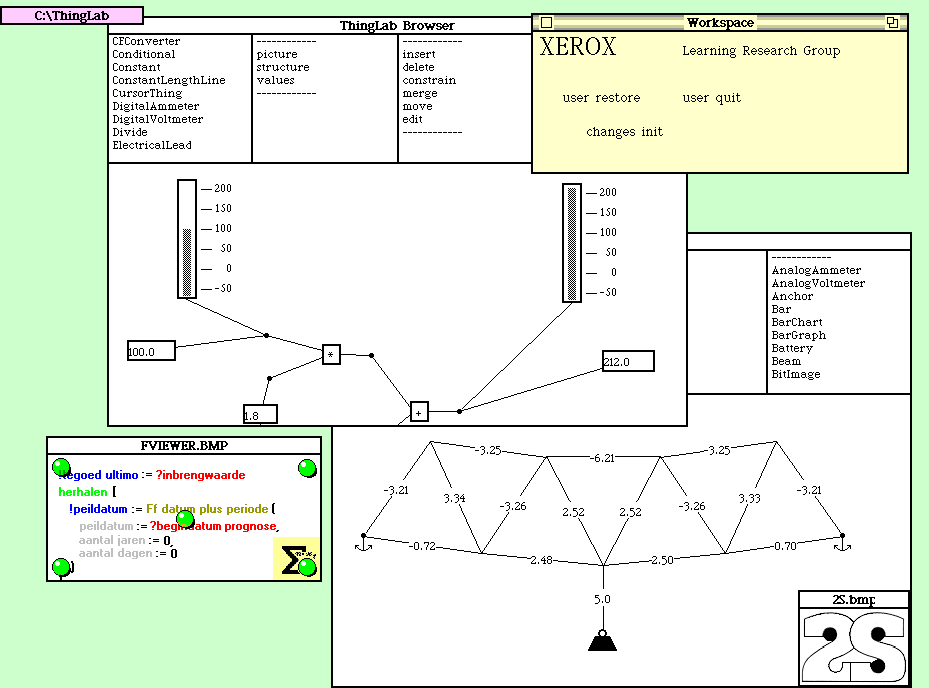
\includegraphics[width=0.6\textwidth]{thinglab.png}           
  \end{center}
\end{frame}

\subsection{Interactive geometry}
\begin{frame}{Cabri Geometer, 1986\cite{laborde86}}
  First interactive geometry system dedicated to
  education in mathematics. \\
  A top-down approach to describe the relations among the parts.
  \begin{center}
    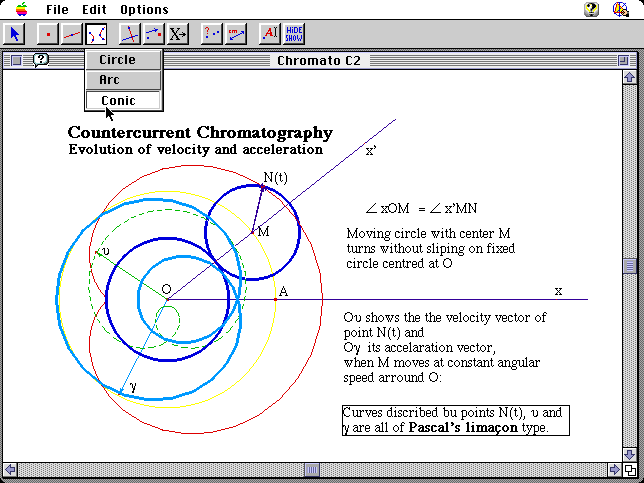
\includegraphics[width=0.6\textwidth]{cabri.png}           
  \end{center}
\end{frame}

\begin{frame}{\drgeo, 1998\cite{drgeo,fernandes98}}
  First interactive geometry system for GNU/Linux,
  enhanced with a touch of end-user programming.
    \begin{center}
    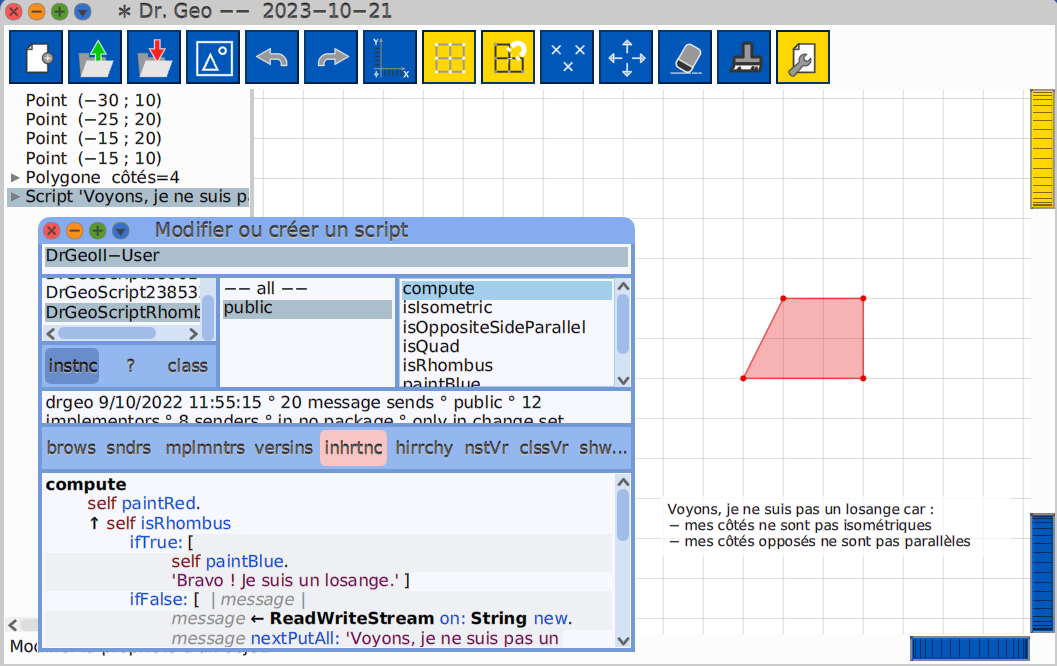
\includegraphics[width=0.7\textwidth]{drgeoScript.png}           
  \end{center}
\end{frame}

\section{Geometric system, Smalltalk approach}
\subsection{What is interactive geometry?}
\begin{frame}
  \begin{itemize}
  \item A collection of math objects -- items -- in a child-parents
    relation
  \item A child depends on its parents. \\
    Example:
    \begin{enumerate}
    \item \textbf{Child}. A point, \emph{middle} of a segment
    \item \textbf{Parent}. A segment with liberty of movement.
    \item \textbf{Dragging child.} \textcolor{red}{\xmark} child stuck as a middle
    \item \textbf{Dragging parent.} \textcolor{green}{\cmark} child
      updated accordingly to keep its property of middle of the
      segment
    \end{enumerate}
  \end{itemize}
\end{frame}
%
\begin{frame}
  \begin{center}
    \beamerbutton{\textbf{DEMO}}
  \end{center}
\end{frame}
%
\begin{frame}{Demo contents}
  \begin{enumerate}
  \item segment, middle  $\rightarrow$ drag segment
  \item segment (one extremity constrained), middle $\rightarrow$ drag segment, observe
  \item segment, perpendicular bisector $\rightarrow$ reverse drag the line, observe
  \item triangle with one vertex ``A'' on a circle $\rightarrow$ drag circle
  \item elaborate previous with constructed altitude (3), construct H
    $\rightarrow$ what are the positions of ``H''
  \item elaborate previous with locus of ``H'' when ``A''
  \item Locus and script
  \end{enumerate}
\end{frame}

\section{DSL -- Kids programming}
\subsection{Describe sketch with code}
\begin{frame}{Why describing a sketch with code?}
  \textcolor{red}{\emph{Point \& Click}} is cool, it hides complexity.\\
  \textbf{Nevertheless:}
  \begin{itemize}
  \item We may want it (complexity) back, to elaborate on the math
    underneath i.e. coordinates system.
  \item Describe a sketch as a text. How can be described a segment?
    Think of its mathematical nature.
  \item Capitalize on the programming features
  \item Growing in complexity, difficult to achieve with
    \textcolor{red}{\emph{Point \& Click}}.
    \begin{itemize}
    \item Constructing hundred of items
    \item Grouping items in collection to apply arbitrary transformation
    \item ...
    \end{itemize}
  \end{itemize}
\end{frame}
%
\subsection{Lesson 1}
\begin{frame}[fragile]{Declarative with sent messages\cite{lesson1}}
\begin{columns}[t]
  \begin{column}{0.5\textwidth}
    Type-in program...
    \vspace*{10pt}
    \fontsize{9pt}{8pt}\selectfont
    \begin{lstlisting}[language=Smalltalk]
DrGeoSketch new
   axesOn;
   gridOn;
   segment: 0 @ 0 to: 6 @ 0;
   segment: 6 @ 0 to: 4 @ 5;
   segment: 4 @ 5 to: 0 @ 0.
 \end{lstlisting}
\end{column}    
    \begin{column}{0.5\textwidth}
      ...to get this sketch
      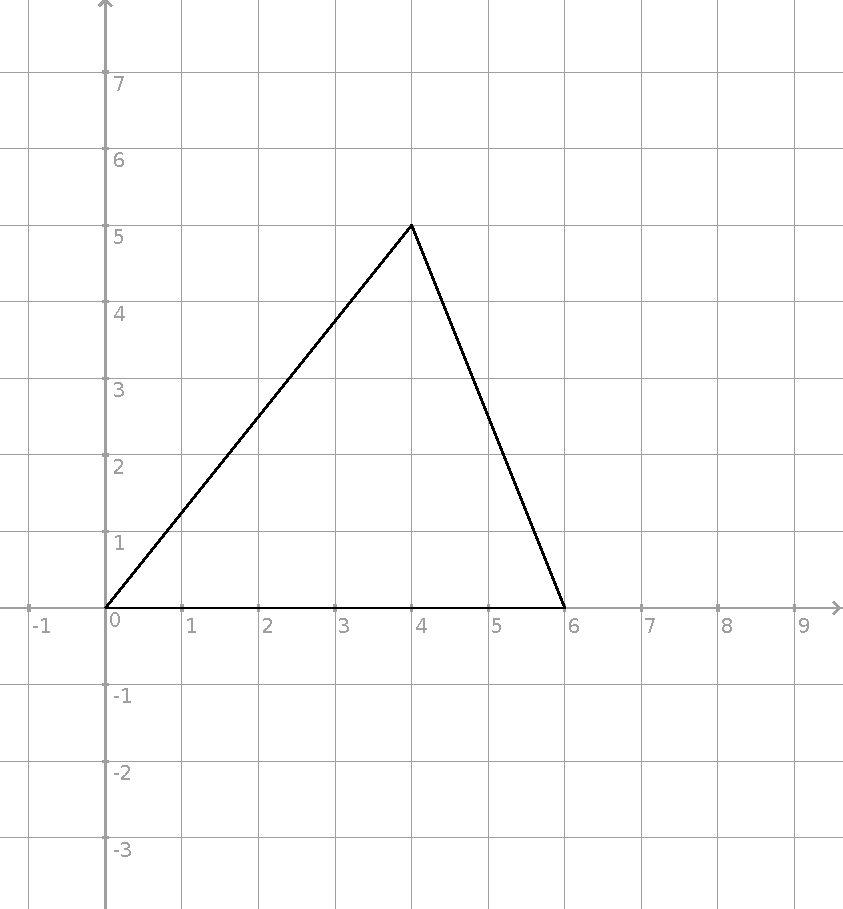
\includegraphics[width=0.9\textwidth]{lesson1.pdf}
    \end{column}  
  \end{columns}  
\end{frame}
%
\begin{frame}{Challenges \& Glossary}
\begin{center}
  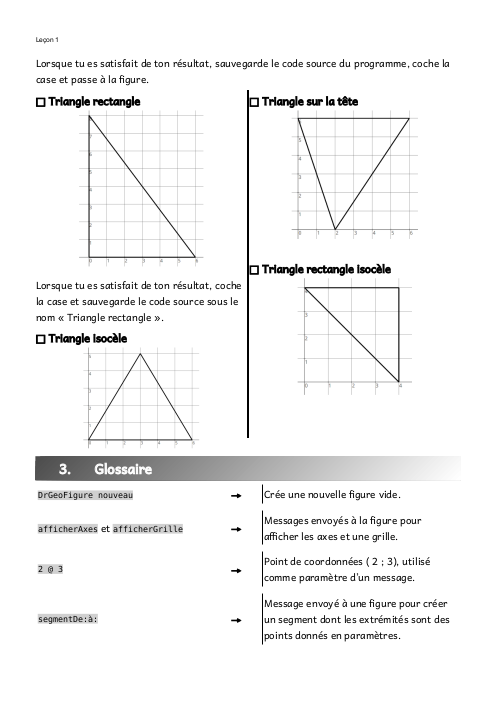
\includegraphics[width=0.5\textwidth]{Triangle2.png}
\end{center}  
  
\end{frame}
\subsection{Lesson 2}
\begin{frame}[fragile]{Introduce variable\cite{lesson2}}
\begin{columns}[t]
  \begin{column}{0.5\textwidth}
    Type-in program...    
    \vspace*{10pt}
    \fontsize{9pt}{8pt}\selectfont
      \begin{lstlisting}[language=Smalltalk]
| sketch |
sketch := DrGeoSketch new.
sketch axesOn; gridOn.
sketch segment: 0 @ 0 to: 8 @ 0.
sketch segment: 8 @ 0 to: 8 @ 5.
sketch segment: 8 @ 5 to: 0 @ 5.
sketch segment: 0 @ 5 to: 0 @ 0
\end{lstlisting}
      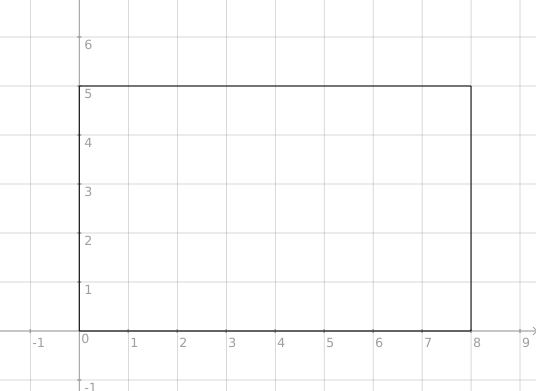
\includegraphics[width=0.8\textwidth]{lesson2.png}
\end{column}
\begin{column}{0.5\textwidth}
  ...then do the challenges 
      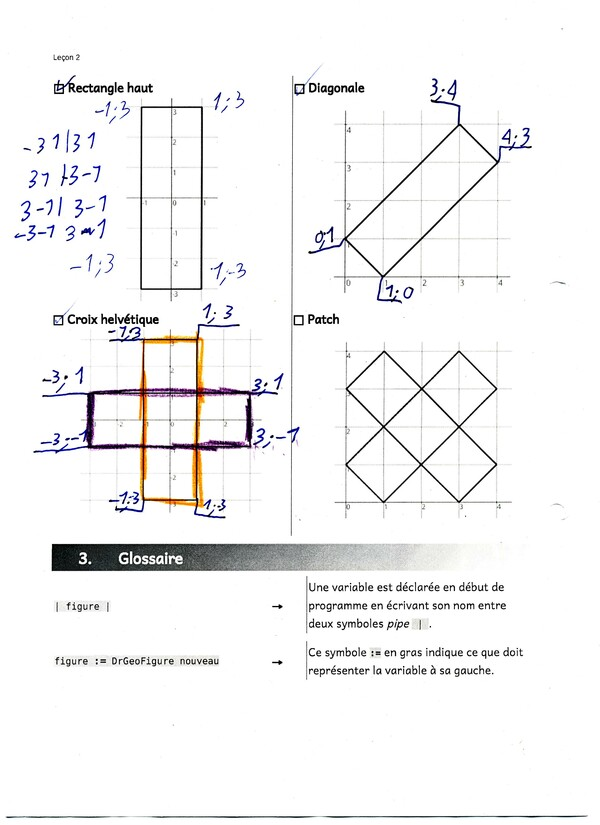
\includegraphics[width=\textwidth]{lesson2Challenges.jpg}
    \end{column}  
  \end{columns}  
\end{frame}

\subsection{Lesson 3}
\begin{frame}[fragile]{Use variables}
  \begin{columns}[t]
    \vspace*{10pt}
    \begin{column}{0.5\textwidth}
      Type-in program...
      \vspace*{10pt}
      \fontsize{9pt}{8pt}\selectfont
    \begin{lstlisting}[language=Smalltalk]
| sketch w h |
h := 3.
w := 8.
sketch := DrGeosketch new.
sketch axesOn ; gridOn.
sketch segment: 0 @ 0 to: w @ 0.
sketch segment: w @ 0 to: w @ h.
sketch segment: w @ h to: 0 @ h.
sketch segment: 0 @ h to: 0 @ 0.
    \end{lstlisting}
\end{column}
\begin{column}{0.5\textwidth}
  ...and kid analysis
      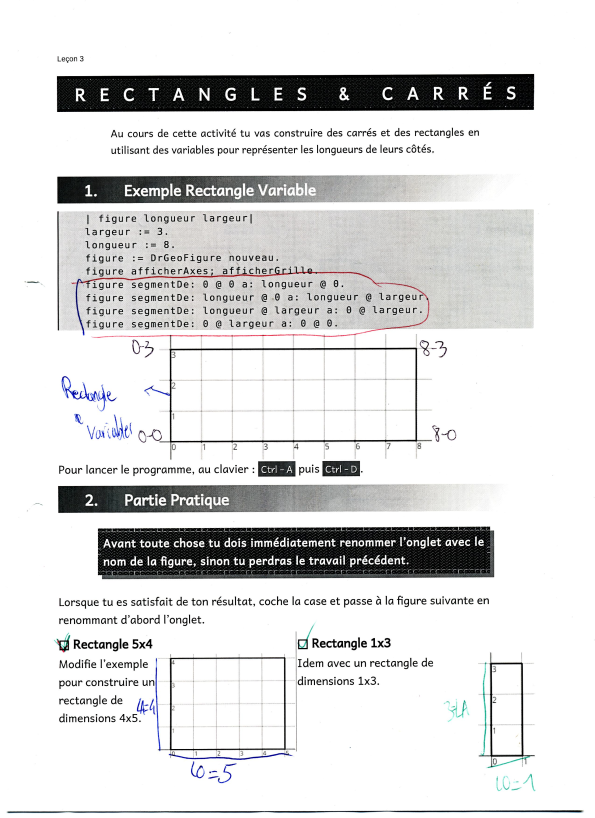
\includegraphics[width=0.9\textwidth]{lesson3Analysis.png}
    \end{column}  
  \end{columns}  
\end{frame}

\subsection{Lesson 5}
\begin{frame}{Compute with loop}
  The \drgeo\ kid IDE
  \begin{center}
    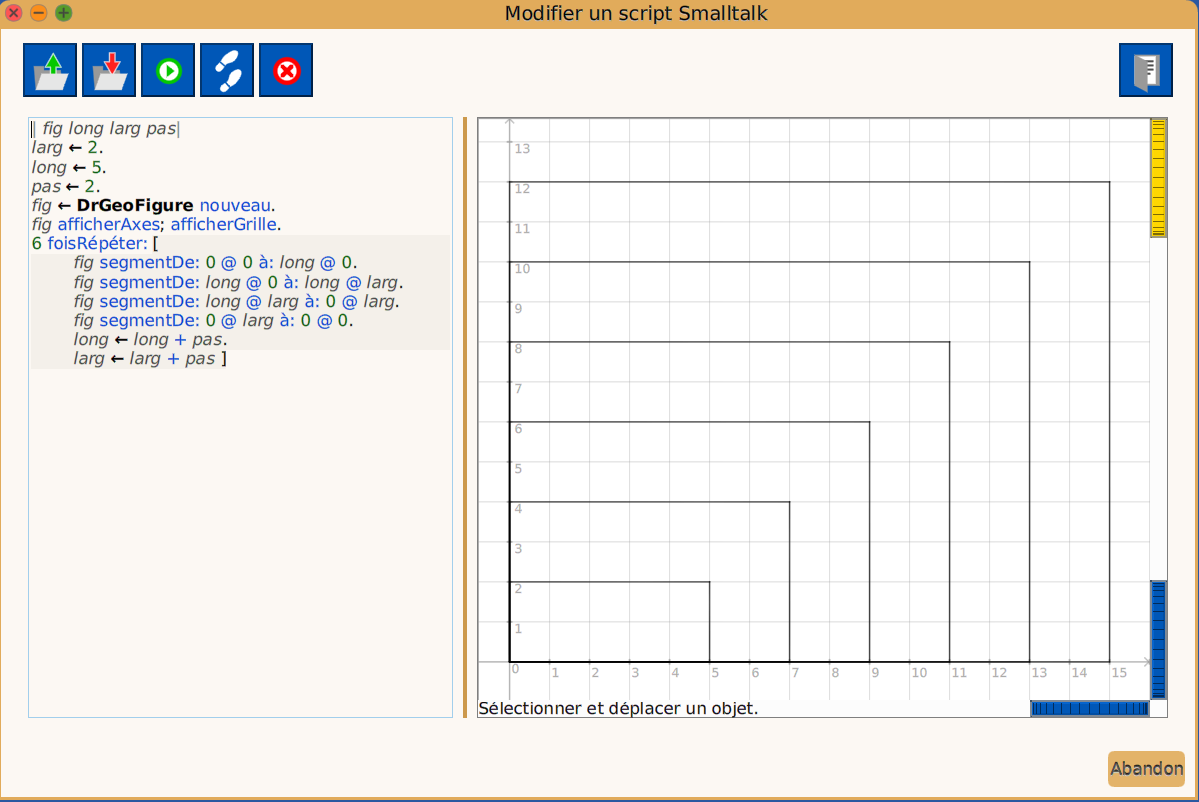
\includegraphics[width=0.8\textwidth]{drgeoKidIDE.png}
  \end{center}
\end{frame}

\subsection{Lesson 6}
\begin{frame}[fragile]{Explore mathematics}
  \begin{columns}[c]
    \begin{column}{0.5\textwidth}
      Regular polygon \& transformation
      \vspace*{10pt}
      \fontsize{9pt}{0pt}\selectfont
      \begin{lstlisting}[language=Smalltalk]
| sketch ptA ptB seg angle |
sketch := DrGeoSketch new.
sketch axesOn; gridOn.
angle := 120.
ptA := sketch point: 3 @ 0.
ptB := sketch
   rotate: ptA
   center: 0 @ 0
   angleDegrees: angle.
seg := sketch segment: ptA to: ptB.
2 timesRepeat: [
   seg := sketch
      rotate: seg
      center: 0 @ 0
      angleDegrees: angle].
(sketch segment: 0@0 to: ptA) small; dotted.
(sketch segment: 0@0 to: ptB) small; dotted        
      \end{lstlisting}
    \end{column}
    \begin{column}{0.5\textwidth}
      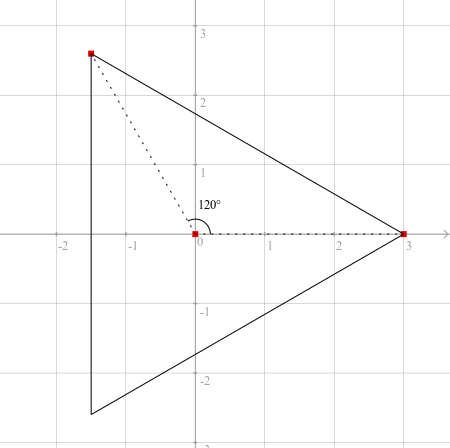
\includegraphics[width=0.6\textwidth]{lesson6.png}
    \end{column}
  \end{columns} 
\end{frame}
%
\begin{frame}{Challenges of regular polygons}
  Measures with protractor...
  \begin{center}
      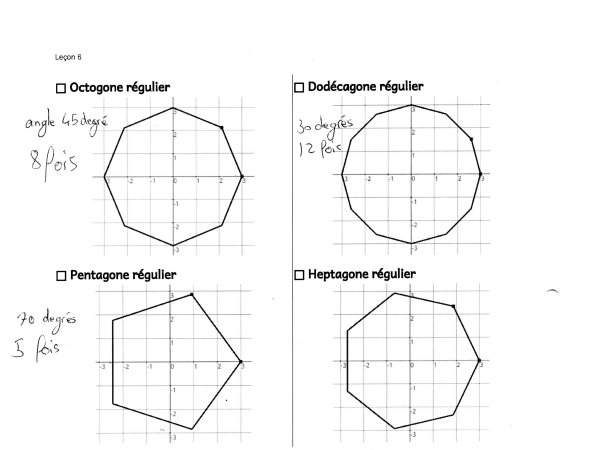
\includegraphics[width=0.8\textwidth]{lesson6-2.png}
  \end{center}
\end{frame}
%
\begin{frame}[fragile]{Houston, we've had a problem here!}
  ...mathematics to the rescue
  \begin{columns}[c]
    \begin{column}{0.5\textwidth}
      \fontsize{10pt}{0pt}\selectfont
      \begin{lstlisting}[language=Smalltalk]
| sketch ptA ptB seg angle |
sketch := DrGeoSketch new.
sketch axesOn; gridOn.
angle := 360 / 5.
ptA := sketch point: 3 @ 0.        
      \end{lstlisting}
    \end{column}
  \begin{column}{0.5\textwidth}
      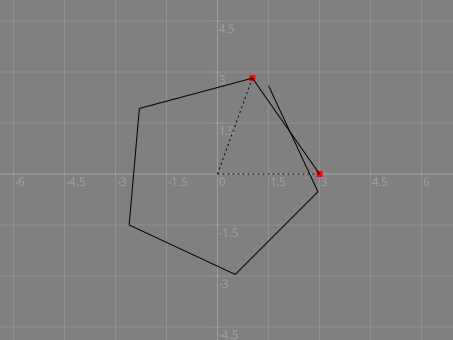
\includegraphics[width=0.9\textwidth]{pentagone.png}
  \end{column}  
\end{columns}
\end{frame}

\subsection{Lesson 9}
\begin{frame}{The benefit of collection}
  \begin{center}
  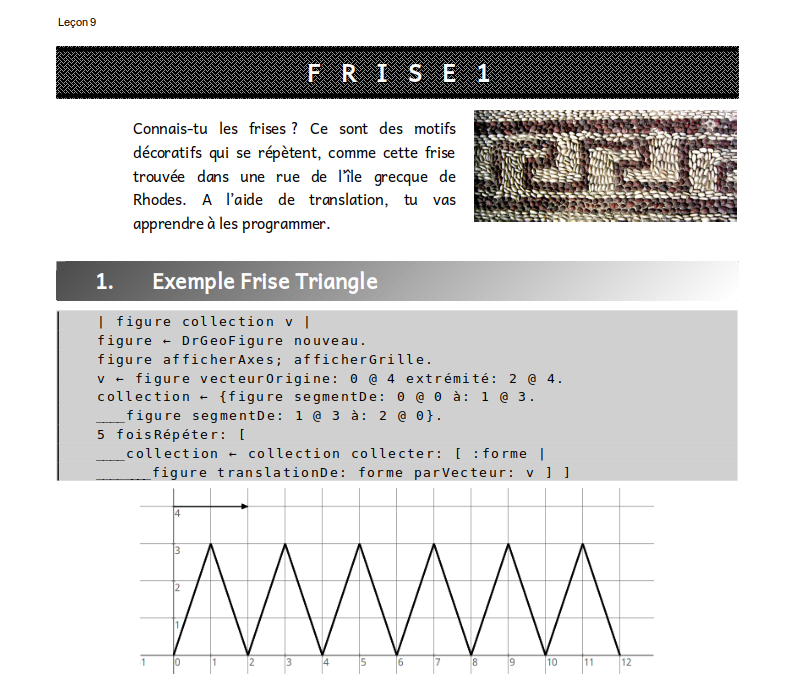
\includegraphics[width=0.75\textwidth]{Frise1a.png}
\end{center}
\end{frame}

\subsection{Final words}
\begin{frame}
  \begin{spacing}{1.5}
  \begin{itemize}
  \item Design a DSL related to a taught domain, \emph{\drgeo} DSL \\
    \tip\ vocabularies of the taught domain
  \item Makes DSL closes to the learner representations, \emph{geometric idioms} \\
    \tip\ DSL in native language. Easy with Smalltalk.
  \item Learn from examples, \emph{Human copies by-design!} \\
    \tip\ learner type-in code, do not elude this part
  \item Conceive challenges \\
    \tip\ progressive, challenge the learner domain
    knowledge (i.e pentagon and heptagon)
\end{itemize}
\end{spacing}

  
\end{frame}
\section{References}
\begin{frame}
  \fontsize{10pt}{8pt}\selectfont
  \begin{thebibliography}{99}

  \bibitem{borning79}
    Alan \textsc{Borning}.
    \href{http://esug.org/data/HistoricalDocuments/ThingLab/ThingLab-index.html}{\emph{Thinglab -- A constraint Oriented Simulation Laboratory.}} Xerox PARC, 1979.

  \bibitem{drgeo}
    Hilaire \textsc{Fernandes}
    \href{https://www.gnu.org/software/dr-geo/}{\emph{GNU \drgeo.}} Free Software Foundation, 1998-2013
    
  \bibitem{fernandes98}
    Hilaire \textsc{Fernandes}
    \href{https://www.gnu.org/software/dr-geo/a_brief_history_of_GNU_DrGeo.html}{\emph{A Brief History of GNU \drgeo.}} Free Software Foundation, 1998
    
  \bibitem{laborde86}
    Jean-Marie \textsc{Laborde}.
    \href{http://www.cabri.net/cabri2/historique-e.php}{Cabri history.} Cabrilog, 2007

  \bibitem{lesson1}
    Hilaire \textsc{Fernandes}
    \href{https://gnu-drgeo.blogspot.com/2023/10/programmer-geometrie-lecon-1.html}{\emph{Programmer Géométrie - Leçon 1.}} 2020, 2023

      \bibitem{lesson2}
    Hilaire \textsc{Fernandes}
    \href{https://gnu-drgeo.blogspot.com/2023/10/programmer-geometrie-lecon-2.html}{\emph{Programmer Géométrie - Leçon 2.}} 2020, 2023

    
  \end{thebibliography}
\end{frame}

\end{document}
